\documentclass[]{beamer}

\usepackage[compatibility=false]{caption}
\usepackage{amsmath}
\usepackage{amssymb}
\usepackage{subcaption}
%\usepackage{sidecap}
%\usepackage{minted}
\usepackage{hyperref}
\usepackage{filecontents}
\usepackage{enumitem}
\usepackage{graphicx}
% -- tikz
\usepackage{
tikz,
pgfplots,
pgfplotstable,
ifthen,
}
\usepgfplotslibrary{patchplots}
\usetikzlibrary{fit}
\usetikzlibrary{calc}
\usetikzlibrary{shapes.geometric}
\pgfplotsset{compat=1.15}
\tikzset{%
  highlight/.style={rectangle, rounded corners, fill=red!15, draw, fill opacity=0.5, thick, inner sep=0pt}
}
\newcommand{\tikzmark}[2]{\tikz[overlay, remember picture, baseline=(#1.base)] \node (#1) {#2};}
%
\newcommand{\Highlight}[2]{%
    \tikz[overlay, remember picture]{
    \node[highlight, fit=(#1.north west) (#2.south east)] () {};}
}


\usepackage{lmodern}
\usepackage{beamercolorthemefiredrake}
\usepackage{beamerouterthemefiredrake}
%\usepackage{beamerfontthemefiredrake}
%\usepackage{beamerthemefiredrake}
\usepackage{beamerinnerthemefiredrake}
\usepackage{pgfplotsthemetolfiredrake}
\setbeamertemplate{items}[square]

\newcommand{\bs}{\boldsymbol}
\newcommand{\abs}[1]{\left| #1 \right|}
\newcommand{\norm}[1]{\left|\!\left| #1 \right|\!\right|}
\newcommand{\vs}{\vspace{\baselineskip}}
\newcommand{\vsh}{\vspace{0.5\baselineskip}}
\newcommand{\trace}{\textrm{tr}}
\newcommand{\nvs}{\vspace{-\baselineskip}}
\newcommand{\nvsh}{\vspace{-0.5\baselineskip}}
\newcommand{\hs}{\hspace{\textwidth}}
\newcommand{\hsh}{\hspace{0.5\textwidth}}
\newcommand{\nhs}{\hspace{-\textwidth}}
\newcommand{\nhsh}{\hspace{-0.5\textwidth}}
\newcommand{\ol}{\overline}
\newcommand{\dif}{\textrm{d}}
\newcommand{\gradient}{\bs{\nabla}\!}
\newcommand{\divergence}{\bs{\nabla}\!\cdot\!}
\newcommand{\real}{\mathbb{R}}
\newcommand{\complex}{\mathbb{C}}
\newcommand{\D}{\textrm{D}}
\newcommand{\on}{\textrm{on }}
\newcommand{\objname}[1]{\texttt{#1}}
\newcommand{\minus}{\scalebox{0.75}[1.0]{\hspace{2pt}\( - \)\hspace{2pt}}}
\newcommand{\plus}{\scalebox{0.75}[0.75]{\hspace{2pt}\( + \)\hspace{2pt}}}
\newcommand{\card}[1]{|{#1}|}
%\newcommand{\aset}[1]{\textit{#1}} % not work with beamer
\newcommand{\aset}[1]{\mathit{#1}}
\newcommand{\amap}[1]{\mathcal{#1}}
%\newcommand{\anarray}[1]{\textsf{#1}} % not work with beamer
\newcommand{\anarray}[1]{\mathbb{#1}}
\newcommand{\iu}{\mathfrak{i}} % imaginary unit
\newcommand{\threeD}{\textrm{\fontsize{5}{0}\selectfont 3D}}


\pgfmathsetmacro{\tikzscale}{2.}
\pgfmathsetmacro{\tikztridegree}{3}
\pgfmathsetmacro{\tikzsqrtthree}{1.7320508075688772}
\pgfmathsetmacro{\tikzsqrttwo}{1.414213}
\pgfmathsetmacro{\tikzoffx}{1.0}
\pgfmathsetmacro{\tikzoffy}{1.0}
\pgfmathsetmacro{\tikzscale}{0.65}
\pgfmathsetmacro{\tikzoffmeshB}{1.5}
\newcommand{\tikzvarl}{0.5}
\definecolor{amber}{rgb}{1.0, 0.75, 0.0}
\definecolor{armygreen}{rgb}{0.29, 0.33, 0.13}
\definecolor{azure(colorwheel)}{rgb}{0.0, 0.5, 1.0}
\definecolor{awesome}{rgb}{1.0, 0.13, 0.32}
\newcommand{\tikzvarlen}{0.35}
\newcommand{\tikzvarnx}{8}
\newcommand{\tikzvarny}{4}
\newcommand{\tikzvarnxm}{7}
\newcommand{\tikzvarnym}{3}
\newcommand{\tikzvarnxtimestwo}{16}
\newcommand{\tikzvarnytimestwo}{8}
\newcommand{\tikzvarnxtimestwominusone}{15}
\newcommand{\tikzvarnytimestwominusone}{7}
\pgfmathsetmacro{\tikzpictureoffset}{6.0}
\newcommand{\tikzmeshcelllen}{2}
\newcommand{\tikzveccelllen}{0.5}
\newcommand{\tikzveccelllensmall}{0.3}
\newcommand{\tikzrankoffset}{2.5}
    \tikzstyle{point}=[circle, minimum size=0pt,inner sep=0pt]
    \tikzstyle{point1}=[circle, minimum size=0pt,inner sep=0pt,fill=gray!40]
    \tikzstyle{orntarc}=[x radius=\tikzmeshcelllen*.2, y radius=\tikzmeshcelllen*.2]
    \tikzstyle{dof}=[circle,fill,inner sep=1.5pt]
    \tikzstyle{fsnode}=[circle,draw=black,minimum size=8pt,inner sep=0pt,fill=white]
    \tikzstyle{fsnode1}=[circle,draw=black,minimum size=11pt,inner sep=0pt,fill=gray!40]
    \tikzstyle{refnode}=[regular polygon,regular polygon sides=4,draw=black,minimum size=12pt,inner sep=-0em,fill=white]
    %\tikzstyle{topoedge}=[draw=black,ultra thick,shorten <= 0pt,shorten >= 0pt,-stealth]
    \tikzstyle{topoedge}=[draw=black,ultra thick,shorten <= 0pt,shorten >= 0pt]

\definecolor{amber}{rgb}{1.0, 0.75, 0.0}
\definecolor{armygreen}{rgb}{0.29, 0.33, 0.13}
\definecolor{azure(colorwheel)}{rgb}{0.0, 0.5, 1.0}
\definecolor{awesome}{rgb}{1.0, 0.13, 0.32}


\usepackage{xcolor}
\usepackage[utf8]{inputenc}
\usepackage[english]{babel}
\usepackage{minted}
%\usemintedstyle{vim}

\newcommand{\dbtilde}[1]{\accentset{\approx}{#1}}
\newcommand{\pp}[2]{\frac{\partial #1}{\partial #2}} 
\newcommand{\dd}[2]{\frac{\delta #1}{\delta #2}}
\newcommand{\DD}[2]{\frac{D#1}{D#2}}
\newtheorem{remark}{Remark}

%%%%%%%%%%%%%%%%%%%%%%%%%%%%%%%%%%%%%%%%%%%%%%%%%%%%%%%%%%%%%%%%%%%%%%%%%%%%%%%%
\begin{document}
    \title[]
              {Recent Development in \textsf{Firedrake}}
    \author{Koki Sagiyama\inst{1} \and David A. Ham\inst{1}}
    \institute{
        \inst{1}%
        Department of Mathematics, Imperial College London\\
    }
    \date{ICIAM 2023}
\begin{frame}
    \titlepage
\end{frame}
%%%%%%%%%%%%%%%%%%%%%%%%%%%%%%%%%%%
\begin{frame}
\frametitle{}
\begin{figure}[]
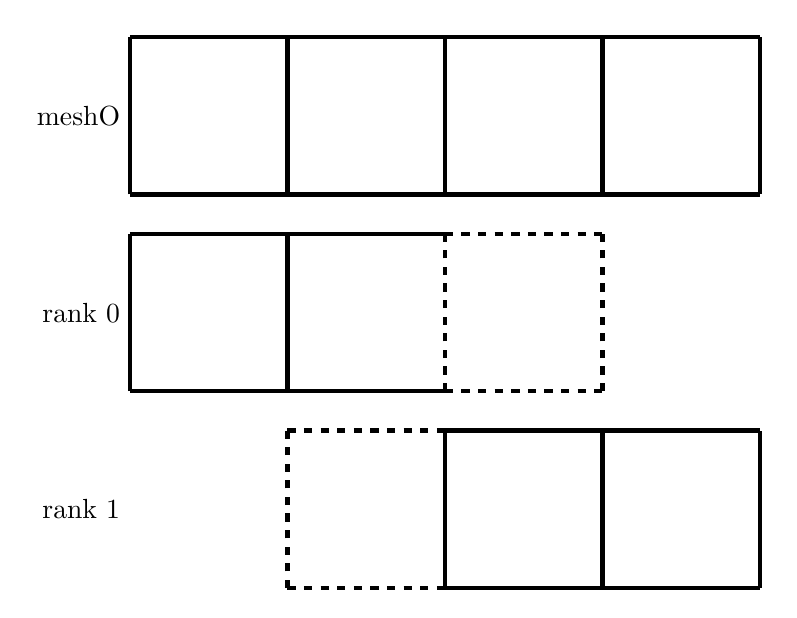
\begin{tikzpicture}
  % Reference element.
  \node[] (p0) [inner sep=0pt] at ($\tikzmeshcelllen*(0, 0)$) {}; % vertices
  \node[] (p1) [inner sep=0pt] at ($\tikzmeshcelllen*(0, 1)$) {};
  \node[] (p2) [inner sep=0pt] at ($\tikzmeshcelllen*(1, 0)$) {};
  \node[] (p3) [inner sep=0pt] at ($\tikzmeshcelllen*(1, 1)$) {};
  \node[] (p4) [inner sep=0pt] at ($\tikzmeshcelllen*(2, 0)$) {};
  \node[] (p5) [inner sep=0pt] at ($\tikzmeshcelllen*(2, 1)$) {};
  \node[] (p6) [inner sep=0pt] at ($\tikzmeshcelllen*(3, 0)$) {};
  \node[] (p7) [inner sep=0pt] at ($\tikzmeshcelllen*(3, 1)$) {};
  \node[] (p8) [inner sep=0pt] at ($\tikzmeshcelllen*(4, 0)$) {};
  \node[] (p9) [inner sep=0pt] at ($\tikzmeshcelllen*(4, 1)$) {};
  \node[] (p10) at ($(p0)!0.5!(p1)$) {}; % facets
  \node[] (p11) at ($(p2)!0.5!(p3)$) {};
  \node[] (p12) at ($(p4)!0.5!(p5)$) {};
  \node[] (p13) at ($(p6)!0.5!(p7)$) {};
  \node[] (p14) at ($(p8)!0.5!(p9)$) {};
  \node[] (p15) at ($(p0)!0.5!(p2)$) {};
  \node[] (p16) at ($(p2)!0.5!(p4)$) {};
  \node[] (p17) at ($(p4)!0.5!(p6)$) {};
  \node[] (p18) at ($(p6)!0.5!(p8)$) {};
  \node[] (p19) at ($(p1)!0.5!(p3)$) {};
  \node[] (p20) at ($(p3)!0.5!(p5)$) {};
  \node[] (p21) at ($(p5)!0.5!(p7)$) {};
  \node[] (p22) at ($(p7)!0.5!(p9)$) {};
  \node[] (p23) at ($(p10)!0.5!(p11)$) {}; % cells
  \node[] (p24) at ($(p11)!0.5!(p12)$) {};
  \node[] (p25) at ($(p12)!0.5!(p13)$) {};
  \node[] (p26) at ($(p13)!0.5!(p14)$) {};
  \foreach \x in {0,1,...,26}
  {
    \node[] (p\x_0) [inner sep=0pt] at ($(p\x)-\tikzrankoffset*(0, 1)$) {};
    \node[] (p\x_1) [inner sep=0pt] at ($(p\x)-\tikzrankoffset*(0, 2)$) {};
  }
  % meshO
  \path[topoedge] ($(p0)$)--($(p1)$);
  \path[topoedge] ($(p2)$)--($(p3)$);
  \path[topoedge] ($(p4)$)--($(p5)$);
  \path[topoedge] ($(p6)$)--($(p7)$);
  \path[topoedge] ($(p8)$)--($(p9)$);
  \path[topoedge] ($(p0)$)--($(p2)$);
  \path[topoedge] ($(p2)$)--($(p4)$);
  \path[topoedge] ($(p4)$)--($(p6)$);
  \path[topoedge] ($(p6)$)--($(p8)$);
  \path[topoedge] ($(p1)$)--($(p3)$);
  \path[topoedge] ($(p3)$)--($(p5)$);
  \path[topoedge] ($(p5)$)--($(p7)$);
  \path[topoedge] ($(p7)$)--($(p9)$);
  % meshO_0
  \path[topoedge] ($(p0_0)$)--($(p1_0)$);
  \path[topoedge] ($(p2_0)$)--($(p3_0)$);
  \path[topoedge, dashed] ($(p4_0)$)--($(p5_0)$);
  \path[topoedge, dashed] ($(p6_0)$)--($(p7_0)$);
  \path[topoedge] ($(p0_0)$)--($(p2_0)$);
  \path[topoedge] ($(p2_0)$)--($(p4_0)$);
  \path[topoedge, dashed] ($(p4_0)$)--($(p6_0)$);
  \path[topoedge] ($(p1_0)$)--($(p3_0)$);
  \path[topoedge] ($(p3_0)$)--($(p5_0)$);
  \path[topoedge, dashed] ($(p5_0)$)--($(p7_0)$);
  % meshO_1
  \path[topoedge, dashed] ($(p2_1)$)--($(p3_1)$);
  \path[topoedge] ($(p4_1)$)--($(p5_1)$);
  \path[topoedge] ($(p6_1)$)--($(p7_1)$);
  \path[topoedge] ($(p8_1)$)--($(p9_1)$);
  \path[topoedge, dashed] ($(p2_1)$)--($(p4_1)$);
  \path[topoedge] ($(p4_1)$)--($(p6_1)$);
  \path[topoedge] ($(p6_1)$)--($(p8_1)$);
  \path[topoedge, dashed] ($(p3_1)$)--($(p5_1)$);
  \path[topoedge] ($(p5_1)$)--($(p7_1)$);
  \path[topoedge] ($(p7_1)$)--($(p9_1)$);
  %
\node[anchor=east] at ($(p10)$) {meshO};
\node[anchor=east] at ($(p10_0)$) {rank 0};
\node[anchor=east] at ($(p10_1)$) {rank 1};
\end{tikzpicture}
\end{figure}
\end{frame}
%%%%%%%%%%%%%%%%%%%%%%%%%%%%%%%%%%%
\begin{frame}
\frametitle{}
Create meshA.

ownership? (interpolate)

\end{frame}
%%%%%%%%%%%%%%%%%%%%%%%%%%%%%%%%%%%
\begin{frame}
\frametitle{}

\begin{align}
V:=V_A\times V_B,
\end{align}

$v:=(v_A, v_B)\in V$
$f:=(f_A, f_B)\in V$


\begin{align}
\int_{\Gamma_{A,\text{interf}}}f_Bv_A\dif\Gamma
\end{align}

\end{frame}
%%%%%%%%%%%%%%%%%%%%%%%%%%%%%%%%%%%
\begin{frame}
\frametitle{}

Locally on each material edge of integration,
it is just like CG1 test function times CG2 trial function, but
entity-DoF maps are defined on different meshes.


\end{frame}
%%%%%%%%%%%%%%%%%%%%%%%%%%%%%%%%%%%%%%%%%%%
\begin{frame}[fragile]
\frametitle{MHD}
\begin{minted}[fontsize=\footnotesize]{python}
from firedrake import *
...
with CheckpointFile("init_cond.h5", "r") as chk:
    mesh = chk.load_mesh("mesh_name")
    f = chk.load_function(mesh, "func_name")

# Define problem.

# Solve for "solution".

with CheckpointFile("solution.h5", "w") as chk:
    f = chk.save_function(solution)
\end{minted}
\end{frame}
%%%%%%%%%%%%%%%%%%%%%%%%%%%%%%%%%%%%
\begin{frame}
\frametitle{}
\begin{figure}[ht]
\begin{tikzpicture}[scale=1]
\begin{axis}[xmin=0, xmax=3,
             ymin=1e-9, ymax=1,
             xlabel={Time},
             ylabel={$F_L$},
             ylabel shift = 0 pt,
             xtick={1,2,3},
             xticklabels={$1$,$2$, $3$},
             legend pos=south west,
             width=7cm,height=7cm]
%\addplot table[x index=0,y index=1,col sep=comma] {convergence_case_2_N_4.dat};
%\addlegendentry{$r=1$}
%\addplot table[x index=0,y index=2,col sep=comma] {convergence_case_2_N_4.dat};
%\addlegendentry{$r=2$}
%\addplot table[x index=0,y index=3,col sep=comma] {convergence_case_2_N_4.dat};
%\addlegendentry{$r=3$}
%\addplot table[x index=0,y index=4,col sep=comma] {convergence_case_2_N_4.dat};
%\addlegendentry{$r=4$}
\end{axis}
\end{tikzpicture}
\end{figure}%
\end{frame}
%%%%%%%%%%%%%%%%%%%%%%%%%%%%%%%%%%%
\begin{frame}
\frametitle{Summary}
\end{frame}
%%%%%%%%%%%%%%%%%%%%%%%%%%%%%%%%%%%%%%%%%%%
\begin{frame}%[allowframebreaks]
\frametitle{References}
\fontsize{5pt}{5}\selectfont
\begin{thebibliography}{Sagiyam,2013}
\bibitem[Ham et al. 2023]{Firedrake}
Ham, D. A., Kelly, P. H. J., Mitchell, L, Cotter, C. J., Kirby, R. C., Sagiyama, K., Bouziani, N., Vorderwuelbecke, S., Gregory, T. J., Betteridge, J., Shapero, D. R., Nixon-Hill, R. W.,Ward, C. J., Farrell, P. E., Brubeck, P. D., Marsden, I., Gibson, T. H., Homolya, M., Sun, T., McRae, A. T. T., Luporini, F., Gregory, A., Lange, M., Funke, S. W., Rathgeber, F., Bercea, G., and Markall, G. R.,
\newblock {F}iredrake {U}ser {M}anual.
\bibitem[PETSc/TAO Users Manual]{petsc-user-ref}
Balay, S., Abhyankar, S., Adams, M. F., Benson, S., Brown, J., Brune, P., Buschelman, K., Constantinescu, E., Dalcin, L., Dener, A., Eijkhout, V., Gropp, W. D., Hapla, V., Isaac, T., Jolivet, P., Karpeev, D., Kaushik, D., Knepley, M. G., Kong, F., Kruger, S., May, D. A., McInnes, L. C., Mills, R. T., Mitchell, L., Munson, T., Roman, J. E., Rupp, K., Sanan, P., Sarich, J., Smith, B. F., Zampini, S., Zhang, H., Zhang, H., and Zhang, J.,
\newblock {PETSc/TAO} Users Manual,
\newblock ANL-21/39 - Revision 3.17 (2022).
\bibitem[Aln\ae{}s et al. 2014]{UFL}
Aln\ae{}s, M. S. Logg, A., \O{}lgaard, K. B., Rognes, M. E., and Wells, G. N.
\newblock {U}nified form language: {A} domain-specific language for weak formulations of partial differential equations,
\newblock ACM Transactions on Mathematical Software. 40(2014) 1--37.
%\bibitem[Homolya and Ham 2016]{Homolya2016}
%Homolya, M. and Ham, D. A.,
%\newblock {A} parallel edge orientation algorithm for quadrilateral meshes,
%\newblock SIAM Journal on Scientific Computing. 38(2016) S48--S61.
\bibitem[Scroggs et al. 2022]{Scroggs2022}
Scroggs, M. W., Dokken, J. S., Richardson, C. N., and Wells, G. N.,
\newblock {C}onstruction of {A}rbitrary {O}rder {F}inite {E}lement {D}egree-of-{F}reedom {M}aps on {P}olygonal and {P}olyhedral {C}ell {M}eshes,
\newblock ACM Transactions on Mathematical SoftwareVolume. 48(2022) 1--23.
\bibitem[Guddati and Lim 2006]{GuddatiLim2006}
Guddati, M. N. and Lim, K.,
\newblock {C}ontinued fraction absorbing boundary conditions for convex polygonal domains,
\newblock International Journal for Numerical Methods in Engineering. 66(2006) 949--977.
%\bibitem[Ainsworth 2004]{Ainsworth2004}
%Ainsworth, M.,
%\newblock {D}ispersive and dissipative behaviour of high order discontinuous Galerkin finite element methods,
%\newblock Journal of Computational Physics. 198(2004) 106--130.
\bibitem[Wimmer and Tang 2022]{Wimmer2022}
Wimmer, G. A. and Tang, X.,
\newblock {S}tructure preserving transport stabilized compatible finite element methods for magnetohydrodynamics, 
\newblock arXiv. 2210.02348(2022).
\bibitem[Sagiyama and Ham 2023]{SagiyamaHam2023}
Sagiyama, K. and Ham, D. A.,
\newblock {A}bsorbing boundary conditions for the Helmholtz equation using Gauss-Legendre quadrature reduced integrations, 
\newblock arXiv. 2308.12255(2023).
\end{thebibliography}
\end{frame}
%%%%%%%%%%%%%%%%%%%%%%%%%%%%%%%%%%%%
\begin{frame}
\frametitle{Acknowledgement}
This work was funded under
%the embedded CSE programme of the ARCHER2
%UK National Supercomputing Service (http://www.archer2.ac.uk) and
the Engineering and Physical
Sciences Research Council [grant numbers EP/R029423/1, EP/W029731/1].
\end{frame}
\end{document}
%%%%%%%%%%%%%%%%%%%%%%%%%%%%%%%%%%%%
